\documentclass{article}
\usepackage[margin=0.5cm]{geometry}
\usepackage[utf8]{inputenc}
\usepackage{graphicx}
\usepackage{listings}
\usepackage{color}
\usepackage{placeins}
\usepackage{hyperref}
\usepackage{xcolor}
\usepackage{caption}
\usepackage{amsfonts}

\begin{document}

\include{frontpage}

\section*{Relations and Partial-Orders:}
Signature:
$$ :) \subseteq S \times S \times \mathbb{R}$$
Relation:
$
\{\emptyset,\emptyset\}, 
\{\emptyset, \{x+1\}\},
\{\emptyset, \{2*y\}\}, 
\{\emptyset, \{z/3\}\}, 
\{\emptyset, \{x+1, 2*y\}\}, 
\{\emptyset, \{x+1, z/3\}\}, 
\{\emptyset, \{2*y, z/3\}\}, 
\{\emptyset, \{x+1, 2*y, z/3\}\},
%%
\{\{x+1\}, \{x+1\}\}, 
\{\{x+1\}, \{x+1, 2*y\}\}, 
\{\{x+1\}, \{x+1, z/3\}\}, 
\{\{x+1\}, \{x+1, 2*y, z/3\}\},
%%
\{\{2*y\}, \{2*y\}\},
\{\{2*y\}, \{x+1, 2*y\}\},
\{\{2*y\}, \{2*y, z/3\}\}, 
\{\{2*y\}, \{x+1, 2*y, z/3\}\},
%%
\{\{z/3\}, \{z/3\}\},
\{\{z/3\}, \{x+1, z/3\}\}, 
\{\{z/3\}, \{2*y, z/3\}\},   
\{\{z/3\}, \{x+1, 2*y, z/3\}\},
%%
\{\{x+1, 2*y\}, \{x+1, 2*y\}\},  
\{\{x+1, 2*y\}, \{x+1, 2*y, z/3\}\},
%%
\{\{2*y, z/3\}, \{2*y, z/3\}\},  
\{\{2*y, z/3\}, \{x+1, 2*y, z/3\}\},
%%
\{\{x+1, z/3\}, \{x+1, z/3\}\},  
\{\{x+1, z/3\}, \{x+1, 2*y, z/3\}\},
%%
\{\{x+1, 2*y, z/3\}, \{x+1, 2*y, z/3\}\},
$

An example of a member of the relation:
<<<<<<< HEAD
$$(\{x+1, z/3\}, \{x+1, z/3\}) \in :)$$
$$\{x+1, z/3\}:)\{x+1, z/3\}$$
An example of a non-member of the relation:
$$(\{x+1, z/3\}, \{x+1, z/3\}) \notin :)$$
$$\{x+1, z/3\}\not:)\{x+1, z/3\}$$
Does the set S and relation $:)$ form a partial-order? Yes. The relation is:\\
\begin{itemize}
	\item Reflexive, every element is related to itself. Example $\{x+1\}\sqsubseteq\{x+1\}$
	\item Antisymmetric, two elements must not be related in both directions. Example $\{x+1\}\sqsubseteq\{x+1, 2*y\}$ but $\{x+1\}\not\sqsubseteq\{x+1, 2*y\}$
	\item Transitive, if the first element is related to the second element, and the second is related to the third, then the first is related to the third. Example $\{x+1\}\sqsubseteq\{x+1, 2*y\}$ and $\{x+1, 2*y\}\sqsubseteq\{x+1, 2*y, z/3\}\}$ then $\{x+1\}\sqsubseteq\{x+1, 2*y, z/3\}\}$
\end{itemize}
Draw a Hasse diagram:
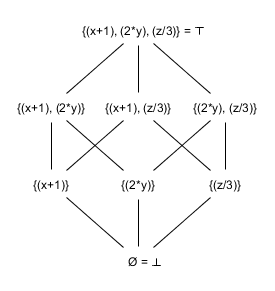
\includegraphics[width=0.5\textwidth]{Hasse}


\section*{Greatest-Lower-Bound:}
Given a lattice $L = (S, \sqsubseteq)$; what do the elements $\sqcup S$ and $\sqcap S$ correspond to? Assuming $S$ from above, $\sqcup S$ is $\{x+1, 2*y, z/3\}\}$, and $\sqcap S$ is $\emptyset$
\section*{Lattices:}
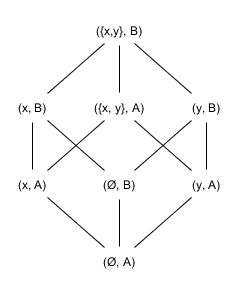
\includegraphics[width=0.5\textwidth]{Lattices}

\noindent A $L_1 \times L_2$ lattice will have $|L_1| * |L_2|$ points. So the resulting lattice will in this case have $2 * 4 = 8$ points.

\end{document}